\subsection{Vertices}\label{sec:vertices}
The problem is modelled as a weighted graph $G = (V, E, w)$. Each vertex is one location the tour must
visit, labelled V0--V9 (Table~\ref{tab:vertices}). V0 is the start and end point. The coordinates locate
each vertex on the map and are used by the divide step: $x$ is the longitude and $y$ is the latitude.

\begin{table}[H]
\centering
\caption{Vertices of the graph: the \NumVertices{} tour locations in Cagayan de Oro City.}\label{tab:vertices}
\vspace{4pt}
\footnotesize
% AUTO-GENERATED by code/main.py --export-latex. Do not edit; re-run the export instead.
\begin{tabular}{l l l r r}
\toprule
\textbf{Vertex} & \textbf{Location} & \textbf{Area} & \textbf{Latitude} & \textbf{Longitude} \\
\midrule
V0 & USTP Cagayan de Oro Campus (start) & C. M. Recto Ave, Lapasan & 8.48607 & 124.65681 \\
V1 & Limketkai Center & Lapasan & 8.48139 & 124.65637 \\
V2 & Centrio Mall & C. M. Recto Ave, Licoan & 8.48483 & 124.65062 \\
V3 & Pelaez Sports Center & Don Apolinar Velez St, Burgos & 8.48180 & 124.64702 \\
V4 & Museo de Oro (Xavier University) & Corrales Ave, Nazareth & 8.47587 & 124.64598 \\
V5 & Divisoria Plaza & Barangay 5, Carmen & 8.47750 & 124.64465 \\
V6 & St. Augustine Metropolitan Cathedral & Gaston Circle, Carmen & 8.47497 & 124.64147 \\
V7 & Port of Cagayan de Oro & Macabalan & 8.49453 & 124.66219 \\
V8 & Liceo de Cagayan University & R. N. Pelaez Blvd, Carmen & 8.48566 & 124.63927 \\
V9 & Capitol University & Corrales Ext, Barangay 25 & 8.48818 & 124.65257 \\
\bottomrule
\end{tabular}

\end{table}

\begin{figure}[H]
\centering
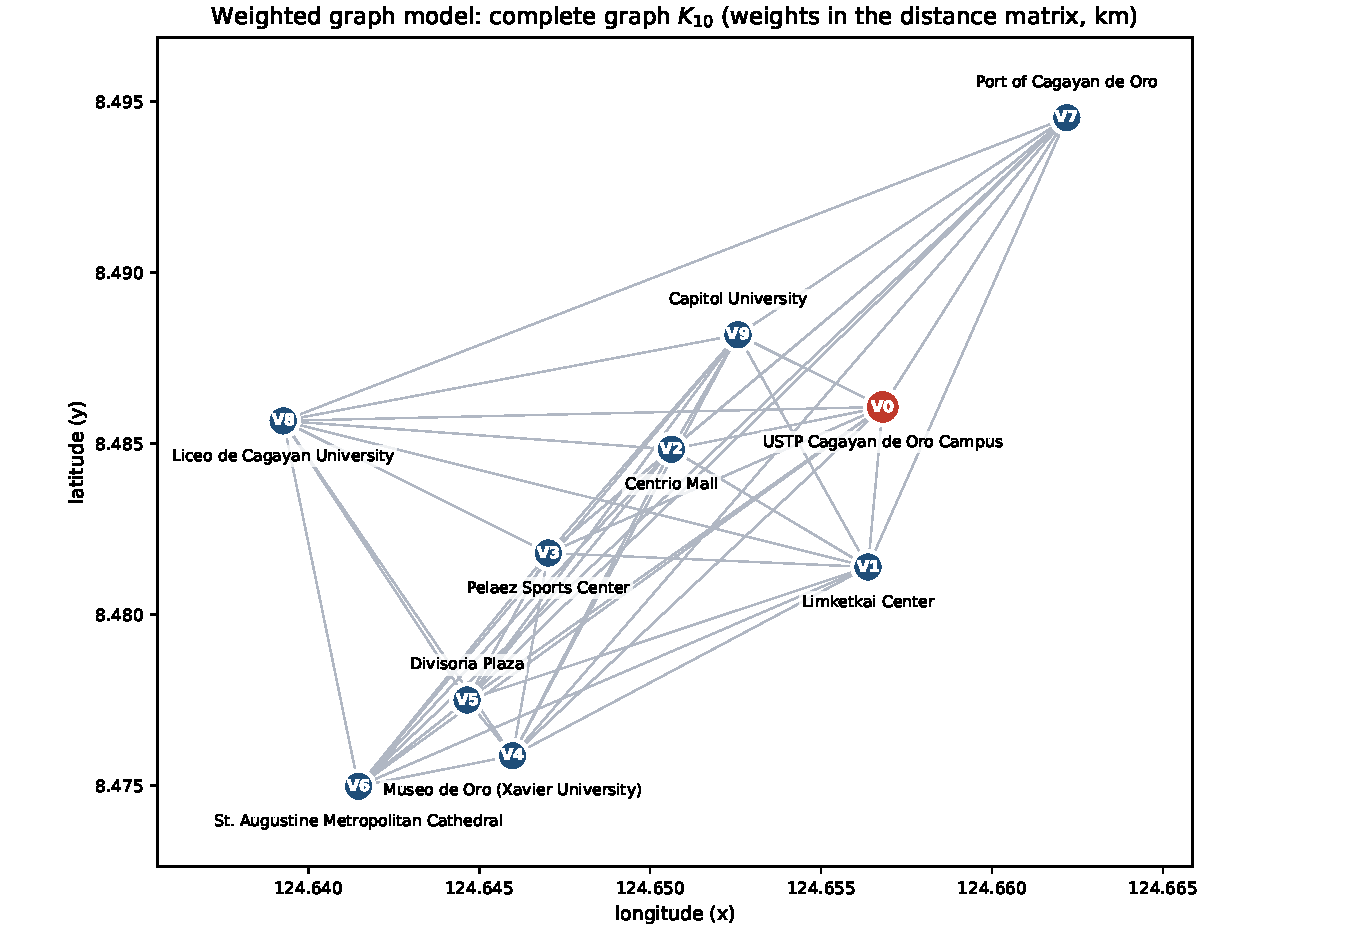
\includegraphics[width=0.85\textwidth]{graph.pdf}
\caption{Labelled graph model of downtown Cagayan de Oro. Every pair of locations is joined by an edge
(complete graph $K_{\NumVertices}$). Edge weights are listed in Table~\ref{tab:matrix}.}\label{fig:graph}
\end{figure}
